\documentclass[11pt,a4paper,twocolumn]{IEEEtran}
\usepackage[utf8]{inputenc}
\usepackage{lipsum}
\usepackage{tabularx, booktabs}
\usepackage{amsmath}
\usepackage{amsfonts}
\usepackage{caption}
\usepackage{pdfpages}
\usepackage[margin=2.5cm]{geometry}
\usepackage{listings,lstautogobble}
\usepackage{amssymb}
\usepackage{hyperref}
\usepackage{graphicx}
\usepackage{svg}
\usepackage{pgf}
\usepackage{array}
\usepackage{cancel}
\usepackage{lipsum}
\usepackage{tikz}

\newcommand*\circled[2][1.6]{\tikz[baseline=(char.base)]{
		\node[shape=circle, draw, inner sep=1pt, 
		minimum height={\f@size*#1},] (char) {\vphantom{WAH1g}#2};}}
\newcommand{\sepline}{\noindent\makebox[\linewidth]{\rule{\textwidth}{1.2pt}}}
\newcommand{\bsepline}{\noindent\makebox[\linewidth]{\rule{7.5cm}{1.2pt}}}
\newcommand{\esepline}{\noindent\makebox[\linewidth]{\rule{7.5cm}{0.5pt}}}

\newcommand{\mysvg}[2]{\includesvg[width=0.#2\linewidth]{../svgs/#1}}
\newcommand*{\Scale}[2][4]{\scalebox{#1}{$#2$}}
\definecolor{RoyalBlue}{cmyk}{1, 0.50, 0, 0}
\lstset{language=Python,
	keywordstyle=\color{RoyalBlue},
	basicstyle=\fontsize{10}{10}\ttfamily,
	commentstyle=\ttfamily\itshape\color{gray},
	stringstyle=\ttfamily,
	showstringspaces=false,
	breaklines=true,
	frameround=ffff,
	rulecolor=\color{black},
	autogobble=true
}

\author{Saverio Monaco, Gerardo Carmona\\ 2012264\hspace{1.5cm} ???????\\ \sepline}
\title{\textbf{Low Pass FIR Filter in FPGA}\\ Management and Analysis of Physics Datasets - MOD. A}


\begin{document}
	\maketitle
	\begin{abstract}
		FIR Filters are a class of filters that are relatively easy to implement in a FPGA. They can be pretty versatile since they can comprehend Low Pass, High Pass, Band Stop and Band Pass filters. In this project we present an example of a Low Pass filter.
	\end{abstract}
	\section{FIR Filter}
	A Filter takes as an input a signal $X[n]$ and outputs a refined one $Y[n]$, for the case of a FIR Filter, the law $X[n]\to Y[n]$ is described as follows: 
	$$ Y[n] = \sum_{i=0}^N C_i x[n-i] $$
	where $N$ is the filter order. This order is totally arbitrary, the higher the order is, the better the filter performs. In this project, we choosed to implement a 3 order filter (4-Taps FIR Filter).\\ Our transformation law is then
	$$\begin{aligned} Y[n]&=\sum_{i=0}^3 C_ix[n-i]=\\ & \Scale[0.8]{\hspace*{.2cm}=C_0x[n]+C_1x[n-1]+C_2x[n-2]+C_3x[n-3]}\end{aligned}$$
	The circuit able to implement this is the following:
	\begin{figure}[h]
		\centering
		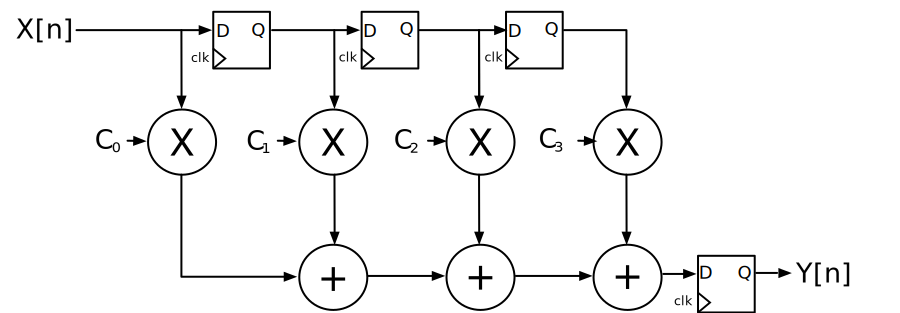
\includegraphics[width=1\linewidth]{img/FIR_direct_svg}
		\caption{Circuit for a FIR Filter}
	\end{figure}\\
	The component represented by a square is a \emph{Flip-flop} (necessary to store the past 3 input for the weighted sum), while \includegraphics[width=0.05\linewidth]{img/x} and \includegraphics[width=0.05\linewidth]{img/+} represent respectively the operations of multiplication and addition.
	\subsection*{The coefficients}
	The value of the coefficients depends on what type of filter do we want to implement and which value of frequencies do we want to filter out.\\
	The values of the coefficients can be computed with \emph{Python} using the function \texttt{firwin} in Scipy:
	\begin{lstlisting}
	from scipy import signal
	
	numtaps = 4
	f = 3
	
	signal.firwin(numtaps, f, fs=125)
	
	[0.04673608 0.45326392 0.45326392 0.04673608]
	\end{lstlisting}
	The coefficients in output will make us build a low pass filter with a cut-off frequency of 3 Hz for a sampling frequency of 125 Hz
	\begin{figure}[h]
		\centering
		\includegraphics[width=0.7\linewidth]{img/lowpass}
		\caption{Low Pass filter}
	\end{figure}
	\section{Implementation of a FIR Filter in VHDL}
	We cannot directly implement the coefficient just found since they are not integers, one way to solve it is to multiplying them before the filtering process and rescaling consequently the output signal. For example:\\$$20\times 0.75 = 15$$ In binary terms it means
	$$ 10100_2 \times 0.11_2 = 1111_2$$
	To realize this, we must scale the quantity $0.11_2$ by multiplying it by $2^Q$ (resulting in a shift of bits) until we obtain an integer, then after the multiplication we can rescale back (shifting to the other direction).
	$$0.11_2 *\times 2^3 = 0.11_2 <<3 = 110$$
	Now we can do the multiplication
	$$10100_2\times 110_2 = 1111000_2$$
	Then we rescale back
	$$1111000_2 >> 3 = 1111_2 = 15$$
	In practice, we needed to scale the coefficients and write them in hexadecimal:
	\begin{lstlisting}
	c = signal.firwin(4, 3, fs=125)
	rc = c * 2**8
	hex_rc = []
	
	for i in range(numtaps):
	hex_rc.append(hex(trunc_rc[i]))
	
	print(rc)    
	print(hex_rc)
	
	[ 11.964 116.035 116.035  11.964]
	['0xc', '0x74', '0x74', '0xc']
	\end{lstlisting}
	\subsection*{The algorithm}
	When you multiply two numbers of N-bit and M-bit the output dynamic of the multiplication result is (N+M)-bits.\\
	When you perform addition, the number of bit of the result will be incremented by 1.\\
	This means that, considering the coefficients being 8 bits wide, if the input signal is 8 bits, the output signal should have 18 bits.\\
	In order to write a code able to compute this operation:
	$$ Y[n] = \sum_{i=0}^N C_i x[n-i] $$
	We implemented 5 processes in it:
	\begin{itemize}
	\item\textbf{p\_input} (initialization): The new value is stored in X[N] and the old ones are shifted one place to the right
	\item\textbf{p\_mult} (multiplication): All the for values X[i] are multiplied by their coefficient $C_i$
	\item\textbf{p\_add\_0} (first additions): The additions $X[N]\times C_0 + X[N-1]\times C_1$ and $X[N-2]\times C_2 + X[N-3]\times C_3$ are performed and stored paying attention in avoiding overflows
	\item\textbf{p\_add\_1} (final addition): The values of the last process are added together as always paying attention to overflows
	\item\textbf{p\_output} (output): The 18 bits output is resized to 8 (same as the input)
	\end{itemize}
\begin{figure}[h]
	\hspace*{-1cm}
	\includegraphics[width=1.2\linewidth]{img/firalg1}
	\caption{Algorithm of FIR Filter}
\end{figure}
	\section{UART implementation}
	A UART is one of the simplest hardware devices capable of transfer data from and to the FPGA.
	To set up a UART correctly, the device and the FPGA must agree on how quickly the data is transfered, this speed is called \emph{Baud rate}.\\
	The data stream is the following:
	\begin{figure}[h]
		\centering
		\includegraphics[width=1\linewidth]{img/baud}
		\caption{UART communication}
	\end{figure}\\
	By default the \emph{Idle state} (the state where the transmitter is waiting for data to send) is \texttt{HIGH}, the \emph{start bit} is \texttt{LOW}, no information is transfered with the start bit, it just tells that some data will be transfered after. Then the bits will be transfered, obviously they can be either 0 or 1, then the end of the stream is announced by the \emph{stop bit} that is \texttt{HIGH}\medskip\\
	The complete project can be schematized as it follows:
	\begin{figure}[h]
		\centering
		\includegraphics[width=1\linewidth]{img/projectcomplete}
		\caption{FPGA structure}
	\end{figure}\\
	Inside the FPGA we will have a \emph{receiver} that will receive data from Python through a USB, the data will be sent to the FIR Filter, it will be filtered and then sent to the transmitter, from there Python can read the output.\\
	For this project we need then 3 main entities: the Fir Filter (already explained), the Receiver and the Transmitter (already provdided). These 3 entities are managed by another entity \emph{top}:
	\begin{figure}[h]
		\centering
		\hspace*{-.8cm}\includegraphics[width=1.1\linewidth]{img/code1}
	\end{figure}\newpage
	\section{Results}
	The results shown are for a signal consisting of two frequencies: 10 Hz and 60 Hz: 
	\begin{figure}[h]
		\centering
		\includegraphics[width=.9\linewidth]{img/rawsig}
		\caption{Raw signal}
	\end{figure}\\
	Implementing a Filter with a cutoff frequency of 30 Hz we get rid of the higher frequency (the noise), obtaining the following result:
	\begin{figure}[h]
		\centering
		\includegraphics[width=.9\linewidth]{img/fpgaresult}
		\caption{FPGA performance}
	\end{figure}\\
	As we can see the output from the FPGA is a signal of a single frequency of 10 Hz as expected. We can also make a comparison between the output from the FPGA and a simulated FPGA in Python using the function
	\begin{lstlisting}
	python_sig = lfilter(c, 1, wave)
	\end{lstlisting}
	Where c is the matrix of the coefficients, wave is the raw signal input:
	\begin{figure}[h]
		\centering
		\includegraphics[width=1\linewidth]{img/fpgapython}
		\caption{Comparison with Python}
	\end{figure}\\
	Since results from the VHDL implementation ran on the FPGA optimally match the ones
	simulated in Python, we conclude that the FIR Filter has been correctly implemented and that it
	efficiently simulates a low-pass filter.
\end{document}